\documentclass{article}
\usepackage{tikz}
% Packages for general formatting and mathematical symbols
\usepackage[utf8]{inputenc} % Encoding of your TeX file (UTF-8 is common)
\usepackage[T1]{fontenc} % Font encoding
\usepackage{amsmath, amssymb, amsthm} % Math packages
\usepackage{geometry} % Customizing page layout
\usepackage{parskip} % Adds spacing between paragraphs
\usepackage[ruled,vlined]{algorithm2e}
% Packages for graphics (optional)
\usepackage{graphicx} % For including images
\usepackage{float} % For precise placement of figures
\usepackage{appendix}
\usepackage{booktabs}
% Title and author information
\title{Project 2}
\author{Jan van Ruijven}

\begin{document}

\maketitle % Display the title/author information

\section*{Question 1}
\subsection*{1}
The first greedy algorithm implemented is based on the average value of the candidates we have seen. The first candidate is never hired, this is because we cannot calculate the average. For all of the other candidates we compare its value $V_i$ to the average value times some multiplier $M_i$. This multiplier could be optimizated, but in this case it is not. The results for this algorithm can be found in table \ref{tab:greedy-average} in the appendix. An overview of the algorithm itself can be found in the appendix at algorithm \ref{Greedy average}. \\ 
The second algorithm implemented keeps track of the highest candidate we have seen so far, if the candidate is the highest we have seen, we hire him or her and else not. An overview of the results of this algorithm can be found in table \ref{tab:greedy-highest} in the appendix. An overview of the algorithm itself can be found in the appendix at algorithm \ref{Greedy highest}. 
\subsection*{2}
In the Q-learning method implemented will keep track of the n-th highest candidate we have at each state, so in state 1 (the first candidate we see), he or her is always the highest candidate. In state 2 we can be looking at the highest or the lowest candidate, at state 3 there are three diffrent possibilities, the candidate is the highest, the middle one, or the lowest. At state 4, there are 4 possiblities etc. When the Q-learning starts we intialize our states with 0's. When we are running the Q-learning algorithm, each time we hire a candidate i and she is the n'th highest, we update state (i,n). We take the candidate if: $v_i / \max_{i} v_i \geq Q(i, n)$
\begin{equation}
	Q(i, n) = Q(i, n) * (1-\alpha) + \alpha * v_i / \max_{i} v_i 	
	\label{eq:State-Update Ex1}
\end{equation}
\subsection*{3}
The algorithm has been tested for values of alpha ranging form 0.01 to 0.2, the resulting Q-values after 100000 iterations can be found in table \ref{tab:data-Q-learning-hiring} in the appendix. Adding random choises to the algorithm had no effect and using the discount factor gamma would result in a bad outcome. Therefore only the values of alpha have been tested, an over view of effect alpha had over itereations can be found in figure \ref{fig:q-learning-results} in the appendix. As can be seen, the value of alpha does not seem to affect the over result that much. 
\subsection*{4}
 The Q-learning strategy does slightly outperform the greedy strategies, as can be seen in table \ref{tab:Q-learning} in the appendix. Even though many of the first decicions made by the agent are completly arbitrarity in the beginning of the training.  
\subsection*{5}
If we look at state (5,3) in this table (index 5 and value 3), this equals 0.79, this would mean that we only hire the third highest candidate out of the 5 we have seen so far, if the value of this candidate divided by the maximum over all candidates we have seen so far is greater or equal than 0.79. An overview of the algorithm can be found in the appendix at algorithm \ref{Q-learning algo}. 
\section*{Question 2}
\subsection*{1}
If we have the following processing times: p = [10, 9, 8, 7, 6, 5, 4, 3, 2, 1] with 4 machines, the greedy heuristic will obtain the following result:  
\begin{enumerate}
	\item = [10, 3, 2]
	\item = [9, 4, 1]
	\item = [8, 5]
	\item = [7, 6] 
\end{enumerate}
This has a maximum completion time of 15. While the following would be optimal, with a completion time of 14:
\begin{enumerate}
	\item = [9, 4, 1]
	\item = [8, 6]
	\item = [3, 10]
	\item = [7, 5, 2] 
\end{enumerate}
\subsection*{2}
The following instance takes more than 5 seconds to reach optimality: 2000 tasks, 50 machine, p values uniformly distributed between 0 and 10. 
\subsection*{3}
The stopping criterion is equal to the number of jobs that we wish to initialize with the greedy heuristic. For example, if we have 2000 jobs and we wish initialize the longest 10\% of jobs with the greedy heuristic, we set the stopping criterion equal to 200, meaning that once we have given the first 200 highest jobs to the machines, we stop and initialize the ILP-solver with the pre-assigned jobs. For the Q-learning, there are 10 diffrent states, each corresponding to the size of the jobs in the instance, the idea is that an instance with larger jobs, would need more pre-processing and vice versa. In each state there are two possiblities, either we pre-process 10\% of the longest jobs, or we pre-process with 2.5\% of the highest jobs. After this decision, we end up in the final state, which is where the ILP-solver will do the rest of the work. This final state will return the MIP-gap, this is because we are dealing with random instances, some of them will have more large processing times than others. Since the MIP-gap should be as low as possible, our agent will take the lowest option of the two. To make sure our agent tries out every option, the epsilon parameter is set to 0.1, such that 10\% of the time we take a completly random option. The states are initialized with 0's.  
\subsection*{4}
The following instances are created to train our agent: 2000 jobs, 50 machines, there are large jobs wich are uniformly distributed from 500 to 600 and there are small jobs uniformly distributed between 0 and 10. The amount of large jobs is decided by taking a random number between 0 and 1, if this random number equal 0.4 for example, this would mean that around 40\% of the jobs are small, and 60\% of the jobs are large.  
\subsection*{5}
The training results can be found in table \ref{tab: Hybrid Q-table} in the appendix. The epsilon value was chosen because blabla.
\subsection*{6}
The hybid appreach does seem to improve the ILP solver so very good blabla.
\subsection*{7}
No real strategy can be found, maybe need more time to train.
\newpage
\begin{appendices}
\section*{Algorithms}

 \begin{algorithm}[ht]
\SetAlgoLined
\KwData{$Hired_i \in {0,1} \quad i = 2 ... 12$\\ $M_i$ = [5, 4, 3, 2, 1.5, 1.25, 1.2, 1.15, 1.1, 1.05, 1, 1]}
\For{i = 2 \KwTo 12}{
    Calculate average over candidates 1 to i\;
    \If{Value of candidate $i >$ Multiplier $i \times$ average $i$}{
        Hire candidate $i$\;
    }
}
\label{Greedy average}
 \caption{Greedy Average Algorithm}
\end{algorithm}

 \begin{algorithm}[ht]
\SetAlgoLined
\KwData{$Hired_i \in {0,1} \quad i = 2 ... 12$\\ Highest = 0}
\For{i = 1 \KwTo 12}{
    \If{Value of candidate $i >$ Highest}{
        Hire candidate $i$\;
	Highest = Value of candidate $i$
    }
}
\label{Greedy highest}
 \caption{Greedy Highest Algorithm}
\end{algorithm}

 \begin{algorithm}[ht]
\SetAlgoLined
    \caption{Q-learning Algorithm}
    \KwIn{Value array $v$, Q-table $Q_{\text{table}}$}
    \For{$\text{episode} \gets 1$ \KwTo $100000$}{
        \For{$i \gets 1$ \KwTo $12$}{
		\If{$\frac{v_i}{\max_{j=1}^{i} v_i} > Q_{\text{table}}$}{
                Hire the applicant for candidate $i$\;
		Update Q-table\;
            }
        }
    }
\label{Q-learning algo}
 \caption{Q-learning Algorithm}
\end{algorithm}

\newpage

\section*{Algorithm Results}
\begin{table}[ht]
    \centering
    \begin{tabular}{@{}cc@{}}
    \toprule
    \textbf{Name} & \textbf{Value} \\ \midrule
    Greedy Average Algorithm Result & 0.81 \\ \bottomrule
    \end{tabular}
    \caption{Results of the Greedy Average Algorithm}
    \label{tab:greedy-average}
\end{table}

\begin{table}[ht]
    \centering
    \begin{tabular}{@{}cc@{}}
    \toprule
    \textbf{Name} & \textbf{Value} \\ \midrule
    Greedy Highest Algorithm Result & 0.82 \\ \bottomrule
    \end{tabular}
    \caption{Results of the Greedy Highest Algorithm}
    \label{tab:greedy-highest}
\end{table}

\begin{table}[ht]
    \centering
    \begin{tabular}{@{}cc@{}}
    \toprule
    \textbf{Name} & \textbf{Value} \\ \midrule
    Q-learning Algorithm Result & 0.83 \\ \bottomrule
    \end{tabular}
    \caption{Results of the Q-learning Algorithm (alpha = 0.19)}
    \label{tab:Q-learning}
\end{table}

\newpage
\section*{Tables}

\begin{table}[ht]
    \centering
    \caption{Q-learning table results (alpha = 0.19)}
    \label{tab:data-Q-learning-hiring}
    \begin{tabular}{|c|c|c|c|c|c|c|c|c|c|c|c|c|}
        \hline
        Candidate & Value \\
        \hline
	1 & 0.0 \\
        2 & 0.85, 0.69 \\
        3 & 0.89, 0.81, 0.60 \\
        4 & 0.93, 0.86, 0.79, 0.68 \\
        5 & 0.95, 0.87, 0.79, 0.74, 0.70 \\
        6 & 0.96, 0.90, 0.91, 0.84, 0.79, 0.72 \\
        7 & 0.94, 0.96, 0.90, 0.93, 0.87, 0.82, 0.79 \\
        8 & 0.94, 0.97, 0.93, 0.92, 0.85, 0.86, 0.87, 0.81 \\
        9 & 0.98, 0.96, 0.98, 0.97, 0.95, 0.91, 0.90, 0.86, 0.79 \\
        10 & 0.98, 0.96, 0.98, 0.97, 0.95, 0.91, 0.90, 0.86, 0.83, 0.79 \\
        11 & 0.99, 0.99, 0.98, 0.98, 0.96, 0.91, 0.90, 0.87, 0.83, 0.79, 0.69 \\
        12 & 0.99, 0.99, 0.98, 0.98, 0.95, 0.94, 0.91, 0.90, 0.86, 0.78, 0.76, 0.71 \\
        \hline
    \end{tabular}
\end{table}

\begin{table}[ht]
\centering
\caption{Hybrid approach}
\label{tab: Hybrid Q-table}
\begin{tabular}{|c|c|c|}
\hline
State & MIP-gap 2.5\% & MIP-gap 10\% \\
\hline
1 & 0.02 & 0.04 \\
2 & 0.03 & 0.04 \\
3 & 0.03 & 0.05 \\
4 & 0.07 & 0.02 \\
5 & 0.05 & 0.06 \\
6 & 0.06 & 0.06 \\
7 & 0.09 & 0.06 \\
8 & 0.11 & 0.14 \\
9 & 0.12 & 0.22 \\
10 & 0.69 & 0.42 \\
\hline
\end{tabular}
\end{table}

\newpage
\section*{Figures}
\begin{figure}[h]
    \centering
    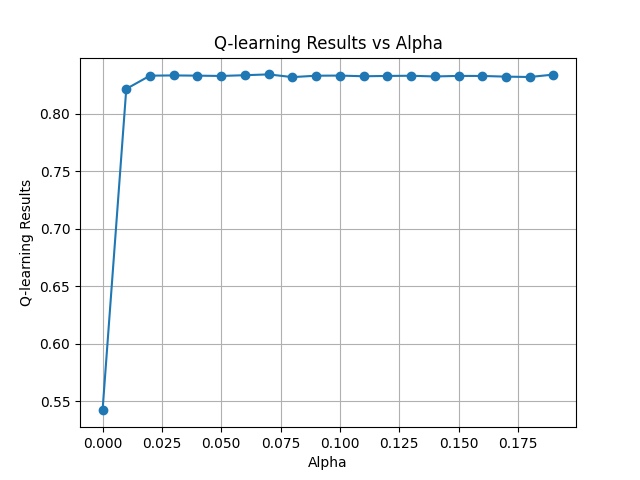
\includegraphics[width=\linewidth]{Q_learning_results.png}
    \caption{Q-learning Results}
    \label{fig:q-learning-results}
\end{figure}
\end{appendices}
\end{document}

